\chapter{評価}
複数タスクにかかる所要時間に対し被験者の予測とADLoggerの予測の差異を比較した上で,
ADLogger導入によって,行動・意識の変容が生じるかどうか評価する.
本章ではまず評価概要を説明し,実験結果を示す.最後に,評価実験から得られた結果をもとに考察を行う.

\section{評価実験の概要}
本研究における評価実験の概要を述べる.はじめに,評価実験を行う目的を説明する.
ついで,評価実験を行う手順について説明する.

\subsection{評価の目的}
本研究では,複数タスクにかかる所要時間の予測に関して被験者の予測とADLoggerの予測の差異を比較する事,
ADLogger導入によって,時間管理に対する苦手意識・行動への変化が起こる事を目的としている.

\subsection{実験評価手法}
今回の評価実験では,被験者に時間の長さを教示し,その長さを産生させる時間産生法\cite{Oguro1961}\cite{Tayama2018}を慶應義塾大学の学生男女20名に対し平日と休日(またはそれに準ずる日)にそれぞれ3回(合計6回)に渡って実施した.
始めに,被験者は事前に各自保持しているiPhoneにADLoggerをインストールして貰う.

実験は平日と休日(またはそれに準ずる日)は異なる動き・見積もりを行う可能性を鑑み,3回分の平日と休日をそれぞれ1回ずつ以上(計6回)実施した,
被験日はまず行動前に朝実施する日常生活動に関して行動名,行動毎の必要時間予測,タスクを連続で行った時の総合必要時間予測を申告してもらう.
尚,6回の計測を通じて予測を適宜修正できるものとする.
%また,実験期間中はアプリケーションの予測精度を向上させる点及びアプリケーション使用頻度を分析する為,可能な限り被験者は実験用に登録した動作を行う度にアプリケーションに計測して貰った.
その後,web会議ツールであるzoom\cite{zoom}およびADLoggerを用いながら実際に行動して貰い実測値を計測する.
zoomにおいては全ての行動の開始時/終了時に連絡を行い,実験者が総合時間を計測する.
更に被験者はADLoggerを用いて行動毎の時間を計測する.
一定期間後(原則4回目)以降の計測はADLoggerのADLogおよびタイマーのカウントアップ表示を閲覧できる状態にしながら計測して貰う.
最終日にはプリケーションによる定性的効果やアプリケーションの改善点を知る為にインタビューを行う.インタビューにて質問する項目は付録Aにて記載した.

実測値およびアンケートで申告した見積もりとのずれに関して,被験者の休日と平日のタスク幅,見積もりの傾向,見積もりと実測値の精度・正確度,インタビュー内容との関係性によって評価を行った上で,全体の分布を反復測定分散分析(Repeated Measured ANOVA),被験者の精度・正確度の変化の推移の評価によってアプリケーションの効果の評価を行った.更にインタビューにて得られた意見をまとめ記述する.

\section{評価結果}
本節では,本システムの導入後時間管理に対し与える影響について,本評価実験で得られた評価結果を示す.
\subsection{データ数について}
%データ数をテーブル化して表示
\subsection{被験者の見積もりの傾向}
まず被験者20名のうち,最後まで実験に協力し有効なデータが取得できた人は【X名】だった.
下記図\label{fig:result1}からも分かるように,被験者の朝行う行動は多種多様であり及び時間も【平均時間X秒,標準偏差X秒】だった.

インタビューによる発言との比較を実施したところ,見積もりに関する想定も個人差があり,一番起こりやすそうな時間で見積もる人は【X名】で精度,正確度は【〜の様になった】..
一番起こりそうな時間より早い時間で見積もる人は【X名】であり精度,正確度は【〜の様になった】.早い時間を見積もった理由は「早めに申告する事でゆっくり支度してしまう事を防ぐ」と言った趣旨の発言が見られた.
一番起こりそうな時間より遅い時間で見積もる人は【X名】精度,正確度は【〜の様になった】.遅い時間を見積もった理由は「ゆとりを持ちたい」と言った趣旨の発言が見られた.
尚,インタビューでの苦手意識との関連性に関しては,【X名】のうち,【Y名】に時間管理に何らかの苦手意識があった.
時間管理に苦手意識の無い人の特徴として【短時間の準備,実際の時間より多めに見積もる傾向(二群比較)】が見られた.
また,時間管理に苦手意識がある人であっても「自分が本当に守ろうと思えば間に合う場合が多い」と言う供述があった人は【X名】であり【予測時間と実際の時間のずれが少ない(二群比較)】と言う特徴が見られた.

また,タスクそれぞれの時間とは別に【被験者A,被験者B】に関しては余裕を持たせるために別途余白時間(【X分,X分】)を確保し予測を行なっていた.

\begin{figure}
\begin{center}
 \fbox{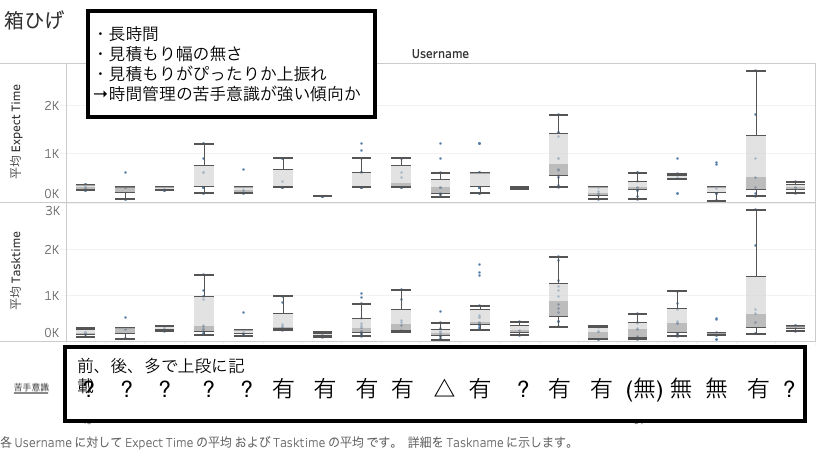
\includegraphics[width=13cm]{images/7/1.png}}
\caption{被験者の準備時間及び見積もり予測の比較}
\label{fig:result1}
  \end{center}
\end{figure}

\subsection{休日と平日のタスク幅}
インタビューの回答について「休日と平日に差が出る」と答えた被験者と「そうで無い」被験者を対象に標準偏差の比較を行ったところ,
休日と平日によって「差が出る」と答えた被験者は「差が出ない」に比較し,【標準偏差の差が大きかった(二群比較)】.
%また苦手意識との関連性は【結果が出そうであれば記述する】.

\subsection{全被験者の見積もり予測の経過について}
総合時間及び一日あたりの平均のずれの時間を反復測定分散分析(Repeated Measured ANOVA)を用いて分析したところ,以下の様になり,
アプリケーションを導入した2回で有意差を【得られなかった】.
\\
(有意水準0.05で帰無仮説を行い,結果を表でまとめて挿入する予定)
尚,時間の調整は【被験者A,被験者B】に見られ,変更したタイミングはそれぞれ下記の様になった.
%テーブルを用いてリストアップして記述


\subsection{実験終了後インタビューについて}
(上記に言及した事以外のインタビューについて〇〇の様な意見が出された等を書いていく予定)

%\subsection{使用頻度について}

\section{考察}
(※詳細は実験データを元に書いていきたいと考えております.一先ず
【】の通りに結果が得られた場合に考えられる考察・Limitationを完結に述べます.)

上記結果から【平日/休日の変化が少ない人が時間管理が得意】である事から,規則正しい生活を送っている人ほどルーティンとして確立しており,ルーティンの習熟度が高い事が分かる.
また,【タスク時間・量の少なさとずれ幅の少なさに相関がある】事から,【行うタスクが短く少ない人ほどずれる時間の幅も少なく時間管理がより容易である】事が分かる.
更にアプリケーションの導入ににより時間を可視化しタスク幅を加味したバッファを加える事によって【精度・正確度の向上が得られた】事から
時間の可視化による時間認識の向上とゆとりのあるスケジューリングの導入が【時間管理能力を向上させる】主要因になる事が分かる.

尚,本実験はデータ数・被験者数が少ない事,短期間である事,一人一人のタスク行動が同一ではない事,時間の見積もり自体は個人間でも均一になりにくい事からデータの偏りが考えられる為更なる収集が必要である.
また,データ数の採集を増やし休日/平日を分けた精度・正確度の評価を行う事でより同一条件下での見積もり幅を策定する事が可能である.
特に,被験者の準備時間が短い程見積もりのずれは少ない傾向がある為他の指標で評価する必要がある.
更に,ずれの評価に関しては見積もりの失敗だけでなく複合的な原因が存在する可能性がある為,今後は本評価手法に限定せずに更なる評価実験が必要になると考えられる.
最後にアンケートにおいてはインタビューによる可能性の示唆を元に今後アンケートなどより統計的に評価しなおす意義があると考える.

\section{まとめ}
本章では,評価実験にの概要及び手法についてまとめたた上で,結果・考察を述べた.
次章では,本研究における今後の展望と本論文のまとめを述べる.
